\section{Opis wykorzystanych technologii}
W tym rozdziale znajdują się informacje dotyczące najważniejszych technologii, które wykorzystano podczas realizacji zadań pracy. W kolejnych podrozdziałach opisane zostały m.in. kody graficzne QR, system mobilny Android oraz Django -- framework do tworzenia aplikacji mobilnych. Na końcu znajduje się opis PayPala, czyli usługi wykorzystywanej do realizacji płatności w systemie.

\subsection{Kody graficzne QR}
Z przedstawianiem danych w postaci kodów graficznych, można się spotkać na przykład w marketach, gdzie towary oznaczane są za pomocą jednowymiarowego kodu kreskowego. Kombinacja jasnych oraz ciemnych linii służy do kodowania informacji, które odczytywane są za pomocą skanera z laserem. Tego typu metody stosuje się głównie w celach identyfikacji. Do przechowywania większej ilości danych wykorzystuje się częściej tzw. kody 2D, do których zaliczy jest kod QR.

Kody QR (ang. Quick Respone - szybka odpowiedź) to dwuwymiarowe, kwadratowe kody graficzne. Składają się z modułów, czyli ciemnych oraz jasnych kwadratów, które są nośnikami danych. Zostały stworzone przez japońską firmę Denso-Wave w 1994 r \cite{thonky_tutorial} i według postanowień licencyjnych, mogą być wykorzystywane bez żadnych opłat. Standard został opisany w normie ISO/IEC 18004:2015 \cite{norma_qr}. Dzięki dodatkowemu wymiarowi, pozwalają na przechowywanie większej ilości informacji (do ok. 7000 liczb lub 4000 znaków alfanumerycznych) niż jednowymiarowe kody kreskowe. Ponadto, zapewniają zdecydowanie lepszą korekcję błędów, ponieważ nawet częściowo uszkodzony kod może zostać poprawnie odczytany. W samym kodzie oprócz danych umieszczane są także miejsca szczególne, ułatwiające orientację podczas odkodowywania. Ich liczba zależy od rozmiaru kodu.

\begin{figure}[h]
	\begin{center}
		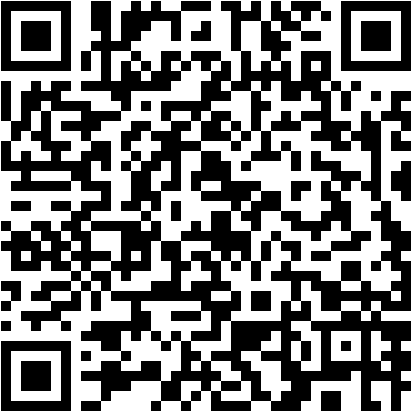
\includegraphics[width=0.2\textwidth]{02/qr_title}
	\end{center}
	\caption{Tytuł pracy przedstawiony w postaci kodu QR.}
	\vspace{-0.3cm}
\end{figure}

Na początku kody QR były głównie wykorzystywane w logistyce, przechowując na przykład informacje o adresie docelowym przesyłki. Współcześnie kojarzone są przeważnie ze smartfonami i można je spotkać niemal wszędzie. Służą do komunikacji z użytkownikami urządzeń mobilnych, przełamując niejako barierę między światem wirtualnym, a rzeczywistym. Mimo, że kod zawiera informacje jedynie w postaci liczb, liter i symboli, to odpowiednie formatowanie informacji pozwala na dodatkowe ich interpretowanie przez urządzenie przenośne. I tak po zeskanowaniu może zostać wysłana wiadomość e-mail, dodany numer do kontaktów, czy wyświetlona strona w przeglądarce internetowej.

\subsubsection*{Sposoby kodowania}

Kodowanie informacji odbywa się w zależności od trzech parametrów, a są to: wersja, typ danych oraz poziom korekcji błędów. Liczba modułów w kodzie ustalana jest przez numer wersji, która jest numerowana od 1 do 40. Determinuje ona ilość informacji, jakie mogą się w kodzie znaleźć. Wersja pierwsza posiada 441 modułów (21 na bok), a czterdziesta składa się z 31329 modułów (177 na bok). Każda kolejna jest większa od poprzedniej o trzy moduły. Wyższy numer wersji przekłada się na większą pojemność kodu, jednak wpływ na to mają także inne parametry. Dla wersji czterdziestej, w zależności od ustawień pozostałych parametrów, liczba znaków mieści się w przedziale od 7089 do 784 znaków.

Typ ustalany jest w zależności od rodzaju danych, jakie mają się znaleźć w kodzie. W przypadku gdy będą to tylko liczby, wystarczający będzie typ numeryczny, jeśli natomiast informacja zbudowana jest także z liter, to użyty może być na przykład typ alfanumeryczny. Wybór wpływa na ilość bitów (czyli modułów), które będą przechowywać informację o pojedynczym znaku, co przekłada się na maksymalną pojemność. Kod QR pozwala na przechowywanie czterech różnych typów danych, a są to:

\begin{itemize}
	\item Numeryczny -- ten tryb pozwala na zakodowanie tylko cyfr od 0 do 9, co umożliwia maksymalnie na przechowywanie 7089 znaków.
	\item Alfanumeryczny -- oprócz cyfr, także wielkie litery oraz znaki '\$', '\%', '*', '+', '-', '.', '/', ':' i spacja. Można zakodować do 4296 znaków. 
	\item Binarny -- domyślnie dla zestawu znaków z ISO-8859-1, ale także UTF-8. Maksymalnie 2953 znaków.
	\item Kanji -- znaki z systemu kodowania Shift JIS. Pomieści nie więcej niż 1817 znaków.
\end{itemize}

Korekcja błędów służy do określenia, czy dane zostały odczytane poprawnie. Pozwala także na odzyskanie części z nich, nawet jeśli kod został uszkodzony (dzięki algorytmowi Reeda-Solomona). Specyfikacja wyróżnia cztery poziomy korekcji. Obok każdego z nich podany został procent danych, jakie można dzięki nim odzyskać:

\begin{itemize}
	\item L (Low) - 7\% danych,
	\item M (Medium) - 15\% danych,
	\item Q (Quartile) - 25\% danych,
	\item H (High) - 30\% danych.
\end{itemize}

\begin{table}[h]
	\caption{Pojemność kodów QR dla różnych ustawień.}
	\vspace{0.3cm}
	\begin{center}
		\begin{tabular}{| c | c | c | c | c | c | c |}
			\hline
			Wersja & Moduły & Korekcja & Numeryczny & Alfanumeryczny & Binarny & Kanji\\
			\hline
			\multirow{4}{*}{1} & \multirow{4}{*}{21x21}&L&41&25&17&10\\
			& & M&34&20&14&8\\
			& & Q&27&16&11&7\\
			& & H&17&10&7&4\\
			\hline
			\multirow{4}{*}{40} & \multirow{4}{*}{177x177}&L&7089&4296&2953&1817\\
			& & M&5596&3391&2331&1435\\
			& & Q&3993&2420&1663&1024\\
			& & H&3057&1852&1273&784\\
			\hline
		\end{tabular}
	\end{center}
\end{table}

Tworzenie kodu graficznego QR jest procesem złożonym. Po analizie danych określającej typ, konieczne jest ich odpowiednie zakodowanie. Informacje dzielone są na bloki, do których dodawane są kolejne bity związane z korekcją błędów. Przed przedstawieniem danych w postaci modułów QR, ważne jest również odpowiednie ich maskowanie. Zbyt duża ilość kwadratów o tym samym kolorze w jednym miejscu, może spowodować błędne odczytanie kodu. Dopiero po tych kilku etapach, może zostać wygenerowany kod. Dla wszystkich najpopularniejszych języków programowania istnieją odpowiednie do tego zadania biblioteki. Na przykład w Pythonie taką biblioteką jest qrcode.

Do odczytywania kodu mogą zostać wykorzystane urządzenia mobilne. Często razem z nimi dostarczane są specjalne aplikacje, które to umożliwiają. Podobnie jak w przypadku kodowania, do odczytywania także można wykorzystać gotowe rozwiązania, w postaci bibliotek. Na urządzenia z systemem Android jest to np.:~bilioteka ZXing (``Zebra Crossing'').

\subsection{Architektura REST}

Porozumiewanie się serwera z urządzeniami mobilnymi w opracowywanym systemie zostało wykonane w oparciu o Representational State Transfer, czyli REST. Jest to wzorzec oprogramowania, opisujący oraz zawierający zalecenia co do tworzenia API w protokole HTTP. Ma w założeniu ułatwić obsługę żądań i odpowiedzi, dzięki czemu nie trzeba zawsze odwoływać do dokumentacji. W jego ramach wykorzystuje się bezstanową komunikację, zasoby, czy hipermedia. Przesyłane dane mogą być w dowolnym formacie, jednak w ostatnim czasie najpopularniejszy jest JSON. Sam REST często jest określany jako następca innego standardu komunikacji -- SOAP.

Adresy URL w przypadku REST pełnią rolę pewnego rodzaju identyfikatora, pod którym kryje się konkretny zasób. Wysyłanie określonych żądań na ten adres, będzie wiązało się z przeprowadzeniem związanych z nim operacji. To jaka operacja będzie wykonywana, zależne jest od metody HTTP określonej w żądaniu, np.: GET -- pobranie danych, PUT -- edycja, POST -- przesłanie nowych danych, DELETE - usunięcie. W REST panuje pewna konwencja co do nazywania adresów URL. Wyróżnia się ich dwa rodzaje, np.: adres /tickets/ będzie się wiązał z dostępem do kolekcji danych, a /tickets/1/ to konkretny element. Wiąże się to bezpośrednio z operacjami, jakie na takich adresach mogą być wykonane. Dodawanie pojedynczego elementu, np.: biletu, będzie wykonywane jako żądanie POST na kolekcji danych. Jednak to są jedynie zalecenia, do których programista nie jest zobowiązany się stosować. Wykorzystanie ich ułatwia jednak interakcję z takim serwisem.

\subsection{System Android}

Systemy na urządzenia mobilne z czasem stawały się coraz bardziej zaawansowane, przypominając swoją funkcjonalnością te przeznaczone na komputery. Dzisiaj oprócz obsługi podstawowych zadań telefonu, jak dzwonienie, pozwalają na przeglądanie internetu, czy instalowanie dodatkowych aplikacji. Do najpopularniejszych systemów w Polsce należą: Android z 65\% udziałem w rynku, Windows Phone - 16\% i iOS - 4\% \cite{polska_jest_mobi}.

\subsubsection*{O Androidzie}

Android to mobilna platforma systemowa, stworzona w 2003~r, a następnie wykupiona przez Google'a w 2005~r. z rąk Android Inc. Od 2007~r. rozwijany jest w ramach sojuszu kilkudziesięciu firm - Open Handset Alliance. Android został zbudowany na bazie jądra Linuksa i podobnie jak on rozpowszechniany jest za darmo w ramach Open Source. To właśnie dostępność oraz możliwość dowolnego modyfikowania spowodowała, że zdołał w tak niedługim czasie zawładnąć rynkiem, stając się najpopularniejszym systemem mobilnym. Można go spotkać na większości popularnych urządzeń przenośnych, jak: telefony komórkowe, smartfony, tablety, netbooki. Jest stosowany także w e-bookach niektórych firm, czy innych sprzętach domowego użytku. 

\subsubsection*{Architektura systemu}
Ze względu na architekturę systemu, można wyróżnić w Androidzie kilka abstrakcyjnych warstw: aplikacji, frameworku aplikacji, bibliotek, środowiska wykonawczego i jądra Linux, na którym bazuje cały system. Cała funkcjonalność systemu, niezbędna podczas działania aplikacji, dostępna jest poprzez framework aplikacji, czyli systemowe API napisane w Javie. Używając go, programista może kontrolować sposób działania oraz wygląd programu. Tutaj znajduje się menedżer aktywności (ang. Activity Manager), odpowiedzialny za cykl życia aplikacji, czy menedżer powiadomień (ang. Notification Manager) obsługujący wyświetlanie wszelkich notyfikacji. Także udostępnianie przez aplikacje swoich funkcjonalności innym programom (z wykorzystaniem intencji) możliwe jest dzięki tej warstwie. Poniżej niej znajdują się natywne biblioteki napisane w C i C++. Dzięki systemowemu API najczęściej nie ma konieczności z nich korzystać, a do tworzenia aplikacji można używać Javy. Najgłębiej w systemie znajduje się jego jądro, czyli Linux. Wykonuje ono najbardziej podstawowe funkcje, będąc odpowiedzialnym m.in. za zarządzanie baterią. Posiada też sterowniki systemowe: ekranu, aparatu, czy audio.

\begin{figure}[h]
	\begin{center}
		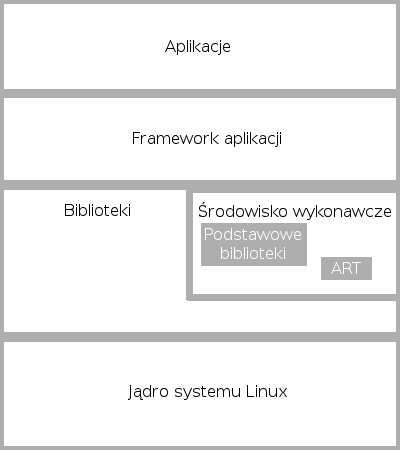
\includegraphics[width=0.5\linewidth]{02/warstwy_android}
	\end{center}
	\caption{Schemat architektury systemu Android.}
\end{figure}

\subsubsection*{Środowisko wykonawcze}
Uruchamianiem programów napisanych w Javie zajmuje się wirtualna maszyna Javy (ang. Java Virtual Machine). Po skompilowaniu tworzony jest kod bajtowy, plik class, który następnie po załadowaniu interpretowany jest przez JVM. Takie podejście pozwala na przenośność programów, czyli niezależność od platformy, kosztem pewnego spadku wydajności.

Mimo, że programy na Androida pisane są w Javie, nie jest wykorzystywany w nim JVM. Głównie jest to spowodowane chęcią stworzenia środowiska uruchomieniowego, które będzie lepiej przystosowane do słabszych wydajnościowo od komputerów maszyn, jakimi są urządzenia mobilne. Proces budowania aplikacji rozpoczyna się tak samo. Kompilator przekształca pliki zawierające kod Javy, do kodu bajtowego. W takiej postaci program nie mógłby zostać jeszcze uruchomiony. Najpierw specjalne narzędzie pod nazwą dx, modyfikuje wynik działania kompilatora. Jego zadaniem jest połączenie wszystkich tych kodów bajtowych w jeden plik dex, usunięcie powtarzających się symboli oraz zamiana znajdujących się tam instrukcji, na odpowiednie dla Androida. Dzięki temu skompilowany program będzie mniejszy oraz z założenia powinien działać szybciej. Ostatnim etapem budowania aplikacji jest stworzenie pliku ze skompilowaną aplikacją oraz jej zasobami.

\begin{figure}[h]
	\begin{center}
		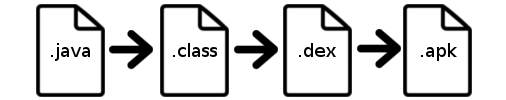
\includegraphics[width=0.5\textwidth]{02/android_dex}
	\end{center}
	\caption{Proces budowy aplikacji.}
	\vspace{-0.5cm}
\end{figure}

Do wersji 4.4 Androida (KitKat) aplikacje uruchamiane były w wirtualnej maszynie Dalvik. Sposób działania był dość zbliżony do JVM, opierając się na interpretacji kodu bajtowego. Jedną z różnic był sposób działania wirtualnego procesora, który w Dalviku opartu został na rejestrach, a nie na stosie. Takie podejście wpływało na mniejsze zużycie pamięci, jednak programy były większe, gdyż instrukcje musiały zawierać dodatkowe informacje co do rejestrów, z których korzystały.

W wersji 5.0 Androida (Lolipop) zastąpiono dotychczasową maszynę wirtualną Dalvik, środowiskiem uruchomieniowym Android runtime (ART). Podobnie jak poprzednik przyjmuje pliki dex, jednak nie interpretuje ich, a w momencie instalacji aplikacji - kompiluje. Taka kompilacja kodu pośredniego języka wysokiego poziomu, do kodu natywnego, nosi nazwę Ahead-of-time (AOT). Przy każdym uruchomieniu aplikacji, dzięki ART, wykorzystywany jest jej natywny kod. Ta zmiana powoduje szybsze działanie i uruchamianie się aplikacji. Wadą jest znacznie dłuższy czas instalacji, który teraz obejmuje także obowiązkową kompilację.

\subsubsection*{Programowanie aplikacji}
Aby móc tworzyć aplikacje na Androida z wykorzystaniem Javy, konieczne jest posiadanie:

\begin{itemize}
	\item Java z JDK i JRE,
	\item Android SDK.
\end{itemize}

Wykorzystując Javę, aplikacja do funkcji systemowych odwoływać się będzie za pomocą udostępnionego przez system API. Dzięki temu, że nie jest to kod natywny, nie jest konieczna osobna kompilacja dla każdej dostępnej architektury. Programy są uniwersalne i dopiero po zainstalowaniu na konkretnym urządzeniu interpretowany jest kod bajtowy, bądź przeprowadzana kompilacja AOT. Przez twórców systemu udostępniane jest także NDK, czyli Native Development Kit. Z jego pomocą aplikacje mogą być tworzone w C lub C++, odwołując się bezpośrednio do bibliotek systemowych. Niestety, mimo możliwego zysku na wydajności, stworzony kod jest zależny od architektury. Dodatkowo większość zewnętrznych bibliotek jest tworzonych w Javie. 

Bardzo zalecane jest używanie zintegrowanego środowiska programistycznego, które automatyzuje niektóre czynności. Potrafi stworzyć za użytkownika projekt z wymaganą strukturą plików, wykonać wszystkie etapy kompilacji, wgrać program na urządzenie i wiele innych. Dedykowanym IDE jest Android Studio, do niedawna wykorzystywany był domyślnie Eclipse.

\begin{figure}[h]
	\begin{center}
		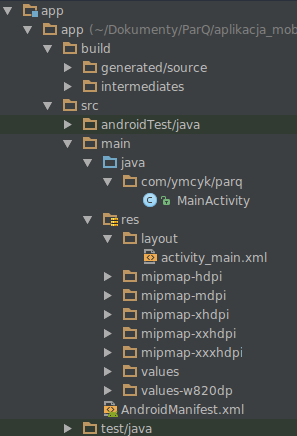
\includegraphics[width=0.25\textwidth]{02/android_pliki}
	\end{center}
	\caption{Pliki projektu utworzonego w Android Studio.}
	\vspace{-0.3cm}
\end{figure}

Podczas działania aplikacja prezentuje użytkownikowi tzw. ekrany. Są to odpowiedniki okien systemowych, gdzie umieszczane są elementy graficznego interfejsu użytkownika, czyli widoki (ang. views), jak np.: przyciski, rozwijane listy, czy pola tekstowe. Wchodząc z nimi w interakcję, możliwa jest komunikacja między użytkownikiem, a urządzeniem. 

Wygląd ekranów definiowany jest w plikach XML, nazywanych układami (ang. layout). Każdy z widoków jest osobnym znacznikiem, a za pomocą argumentów można modyfikować wybrane parametry jak rozmiar, czy kolor. Wszystkie widoki w pliku XML muszą posiadać swojego rodzica, który definiuje jak mają one być traktowane w tym układzie. W Androidzie dostępnych jest ich kilka, a do najpopularniejszych należą: RelativeLayout (położenie widoków określane jest względem siebie), LinearLayout (układ liniowy, gdzie elementy GUI wyświetlane są jeden koło drugiego) i GridLayout (dzieli ekran na siatkę, składającą się z wierszy oraz kolumn, i pozwala umieścić widoki we wskazanych komórkach).

Układy definiują jak dany ekran ma wyglądać, natomiast aktywności (ang. activity), czyli klasy Javy, określają w jaki sposób mają one reagować na interakcje użytkownika. Przechodząc do danego ekranu, tworzona jest najpierw aktywność. Metoda onCreate znajdująca się w aktywności, określa jaki układ ma zostać użyty do zbudowania graficznego interfejsu. W odpowiedzi na interakcję z jakimś widokiem, mp.: przyciskiem, może zostać wywołana metoda znajdująca się w powiązanej z układem aktywności.

Rozwiązania mobilne cieszą się coraz większym zainteresowaniem. Tylko w sklepie z aplikacjami Androida, Google Play, liczba programów przekroczyła w 2015 r. 1,6 mln \cite{biblia_ebiznesu_2}.

\subsection{Framework Django}
Frameworki aplikacji internetowych powstały z myślą o zwolnieniu programisty z obowiązku pisania części kodu, który jest wspólny dla większości serwisów. Może to być dostęp do bazy danych, obsługa linków (ang.~routing), czy zarządzanie sesjami. Dodatkowo, pisanie aplikacji internetowej od podstaw, jest zadaniem czasochłonnym oraz dość trudnym. Frameworki są odpowiedzią na te problemy, dostarczając zestaw gotowych oraz przetestowanych rozwiązań, które należy dostosować do własnych potrzeb. Umożliwiają utworzenie struktury plików projektu, na bazie którego dalej będzie rozwijana aplikacja. Każdy z najpopularniejszych języków programowania oferuje duży wybór silników, przeznaczonych do tworzenia usług internetowych i np.: w C\# napisane zostały ASP.NET i MonoRail, w Javie - Spring i JavaServer Faces, a w Python - Django i Flask. Mogą się różnić przede wszystkim stopniem złożoności, dzięki czemu nadają się do różnych zastosowań - prezentują odmienne sposoby realizacji podobnych zadań.

\subsubsection*{Początki Django}
Django rozwijany jest jako wolne oprogramowanie na GitHub'ie, w ramach fundacji Django Software Foundation, ale skupia wokół siebie także wielu niezależnych twórców. Został napisany w Pythonie, stając się z czasem najpopularniejszym frameworkiem dla tego języka. Jego historia rozpoczęła się w 2003~r., kiedy to dwóch programistów Adrian Holovaty i Simon Willison zaczęli używać Pythona do tworzenia aplikacji webowych dla kilku serwisów informacyjnych, m.in. Lawrence.com. Praca w środowisku dziennikarskim, cechująca się napiętym grafikiem, wymagała niezwykle szybkiej realizacji zadań. Z tej konieczności opracowali własny silnik, który w 2005~r., już pod nazwą Django, został udostępniony publicznie. To właśnie szybkość oraz względna łatwość tworzenia aplikacji są jego głównymi zaletami.

\subsubsection*{Charakterystyka}

Aplikacje Django tworzone są w interpretowanym języku Python, przeznaczonym głównie do pisania skryptów. Jako że jego interpretery dostępne są na wielu platformach, jest on niezależny od systemu operacyjnego. Dodatkowo wsparcie dla wielu paradygmatów (imperatywnego, funkcyjnego, obiektowego), przekłada się na jego szerokie zastosowanie. Oprócz programowania serwerów, jest używany do pisania testów, aplikacji z graficznym interfejsem, a także gier 3D. Wyróżnia się głównie charakterystyczną składnią, w której poszczególne bloki kodu odseparowane są wcięciami (spacje lub tabulator), co wpływa na zwiększoną czytelność.

Architektura aplikacji sieciowych typu klient-serwer, opiera się często na wzorcu projektowym Model-View-Controller (pol.~Model-Widok-Kontroler), w skrócie MVC. Jego ideą jest odseparowanie części prezentacji danych, od kodu odpowiedzialnego za ich przetwarzanie. Aplikacja dzielona jest w nim na trzy główne części. Model jest reprezentacją danych oraz logiki problemu. Widok odpowiedzialny jest za prezentację - określa w jaki sposób informacje mają zostać przedstawione. Kontroler przyjmuje żądania i wykonuje związane z nimi akcje. Głównie aktualizuje widoki oraz modele.

\begin{figure}[h]
	\begin{center}
		\includegraphics[width=0.6\textwidth]{02/MVC_diagram}
	\end{center}
	\caption{Wzorzec projektowy MVC.}
	\vspace{-0.3cm}
\end{figure}

Wzorzec MVC jest stosowany w Django, jednak został zrealizowany w sposób odmienny od najczęściej spotykanych jego implementacji. Z tego względu często nazywa się go wzorcem MTV (Model-Template-View), będącego pewną wariacją MVC. Także wyróżnia się w nim trzy główne części aplikacji, a są to:

\begin{itemize}
	\item Model -- podobnie jak w MVC, zapewnia dostęp do danych. Opisane są tutaj relacje między danymi oraz odbywa się ich walidacja.
	\item Template (pol. szablon) -- warstwa prezentacji, czyli jak ma zostać wygenerowana odpowiedź (w postaci dokumentu HTML lub innym formacie).
	\item View (pol. widok) -- zawiera logikę biznesową. Pobiera dane z modeli i łączy je z szablonami, tworząc w ten sposób odpowiedź. Stanowi pomost między dwoma wcześniej wymienionymi elementami MTV.
\end{itemize}

Rolę kontrolera MVC, pełni w Django sam framework. Otrzymane zapytanie wysyłane jest do odpowiedniego widoku, w zależności od konfiguracji URL.

\begin{singlespace}
	\captionof{listing}{Przykładowa konfiguracja URL w Django.}
	\vspace{0.3cm}
	\inputminted[fontsize=\footnotesize]{python}{src/urls.py}
	\label{l:url}
\end{singlespace}

W przeciwieństwie do mikro frameworków, takich jak Flask, Django dostarcza programiście wielu gotowych rozwiązań, jak: dostęp do baz danych, klasy ORM, obsługa linków URL, uprawnienia użytkowników, automatycznie generowana strona administratora, szablony HTML i wiele innych. Dodatkowo posiada wbudowaną ochronę przed typowymi atakami, takimi jak: cross-site scripting (XSS), cross-site request forgery (CSRF), a także wstrzykiwanie SQL'a.

\subsubsection*{Programowanie aplikacji}

Tak jak większość frameworków, także i Django tworzy za użytkownika gotową strukturę projektu. Poza konfiguracją, nie znajduje się w nim jednak żadna logika. Wszystkie modele oraz widoki w danym projekcie tworzone są w ramach tzw. aplikacji, czyli pakietów Pythona (których struktura także generowana jest przez framework), odpowiednio w plikach models.py oraz views.py. Dzięki temu mogą zostać one ponownie wykorzystane. W hierarchii plików znajdują się na tym samym poziomie, co moduł z konfiguracją projektu. 

\begin{figure}[h]
	\begin{center}
		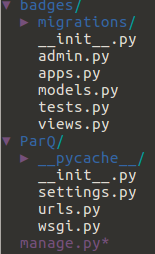
\includegraphics[width=0.15\textwidth]{02/django_structuree}
	\end{center}
	\caption{Struktura plików projektu (ParQ) z aplikacją (badges).}
	\vspace{-0.3cm}
\end{figure}

W pliku settings.py projektu znajdują się wszystkie ustawienia serwisu, takie jak konfiguracja bazy danych, strefy czasowej, silnika szablonów oraz pakietów pośredniczących (middleware) wykorzystywanych np.: do autoryzacji. Tam także powinny zostać zarejestrowane wszystkie aplikacje używane w projekcie.

W models.py aplikacji znajdują się modele danych - są to klasy dziedziczące po Model. Posiadają zmienne klasowe, które reprezentują kolumny w tabelach baz danych. Nazwa takiego pola jest później używana jako nazwa kolumny, natomiast jej typ definiowany jest przez instancję jednej z klas pochodnych od Field. I tak dla przykładu IntegerField będzie typem całkowitoliczbowym, a CharField znakowym. Parametry podane w konstruktorze pozwalają zdefiniować rozmiar, czy unikalność krotki w kolumnie. Relacje również tworzone są za pomocą pól. Model posiadający pole relacji, może odwoływać się za jego pomocą do powiązanych danych. W Django znajdują się trzy takie klasy:

\begin{itemize}
	\item ForeignKey -- pole z kluczem obcym, używane w relacjach jeden do wielu. Tworzona jest kolumna w tabeli.
	\item ManyToManyField -- używane w relacjach wiele do wielu. W bazie danych zostanie automatycznie utworzona tabela pośrednia, z kluczami powiązanych tabel.
	\item OneToOneField -- do relacji jeden do jeden. Także wykorzystywana jest tabela pośrednia, jednakże oba klucze są unikalne - mogą wystąpić tylko w jednej relacji w ramach tej tabeli.
\end{itemize}

W modelach dozwolone jest także definiowanie własnych metod.

\begin{singlespace}
	\captionof{listing}{Przykładowy model danych z modułu models.py.}
	\vspace{0.3cm}
	\inputminted[fontsize=\footnotesize]{python}{src/models.py}
\end{singlespace}

Kolejnym ważnym plikiem w aplikacji tworzonej przez użytkownika jest views.py. To tutaj znajdują się widoki ze wzorca MTV i scalają one szablony z modelami. Jako parametr przyjmują obiekt HttpRequest, zawierający dane zawarte w żądaniu HTTP. To właśnie te widoki podawane są podczas konfiguracji linków w funkcji url, pliku urls.py w projekcie. Zostało to zaprezentowane na listingu \ref{l:url}.

\begin{singlespace}
	\captionof{listing}{Widok.}
	\vspace{0.3cm}
	\inputminted[fontsize=\footnotesize]{python}{src/views.py}
\end{singlespace}

\subsubsection*{Aplikacje jako dodatki}
Napisane aplikacje Django, mogą być wielokrotnie wykorzystywane w innych projektach. Na tej zasadzie funkcjonują dodatki pisane do tego frameworku. Jednymi z nich są: Django REST Framework używany do tworzenia API w architekturze REST, czy django-annoying modyfikujący działanie niektórych elementów silnika.

\subsection{PayPal}

Do realizowania płatności w systemie wykorzystywany jest system PayPal. Jego sposób działania jest nico odmienny od 
pozostałych bramek płatności jakie zostały wymienione w tej pracy, gdyż pełni on także 
funkcję wirtualnej portmonetki. Oznacza to, że pieniądze nie trafiają od razu 
na konto sprzedającego, jak to się dzieje w przypadku PayU, czy Dotpay. 
Zapisywane są najpierw w postaci elektronicznej i dopiero na żądanie mogą 
zostać wypłacone. Wiąże się to niestety z dłuższym czasem oczekiwania i pewną 
prowizją. 

\subsubsection*{Integracja}

Po założeniu konta w PayPalu integracja z tworzonym systemem może odbywać się 
na kilka sposobów. W przypadku sklepów, gdzie płatności realizowane są na 
stronach internetowych, popularnym i najszybszym rozwiązaniem jest PayPal 
Standard Payments. Jest to usługa, która pozwala na wygenerowanie gotowych 
przycisków w postaci fragmentów kodu HTML. Jego kliknięcie przenosi na stronę 
z wyborem metody płatności, a pieniądze przelewane są na powiązane konto 
sprzedającego. Mogą one dotyczyć jednej transakcji, ale możliwa jest także 
obsługa całego asortymentu sklepu. O dokonaniu transakcji i produkcie lub 
usłudze jaka została kupiona, sprzedawca informowany jest za pośrednictwem 
swojego konta na PayPalu.

Powyższy sposób sprawdza się jedynie w przypadku sklepów internetowych. Do 
tworzonego systemu płatnego parkowania, gdzie płatność jest realizowana poprzez 
aplikację na urządzeniu mobilnym, niezbędne jest inne podejście. W tym 
przypadku komunikacja z PayPalem i realizacja, opłat odbywa się za pośrednictwem 
udostępnianego API. Polega ona na wymianie żądań i odpowiedzi z serwerem, 
poprzez protokół HTTP. Może to się odbywać zarówno w architekturze REST, jaki i 
SOAP. Zapytania wysyłane są na domenę api.paypal.com, a komunikacja 
zabezpieczona jest standardem OAuth2.

Pierwszą rzeczą jaką należy wykonać to zarejestrowanie klienta (np.: aplikacji mobilnej), który będzie 
miał prawo obsługiwać płatności w imieniu posiadacza konta PayPal. Dzieje się 
to poprzez utworzenie tzw.~aplikacji (ang. application) w systemie, razem z którą zostanie wygenerowany jego 
identyfikator oraz sekret, w postaci ciągu znaków. Obie te wartości wysłane w 
odpowiednim żądaniu HTTP, pozwolą na uzyskanie tokenu autoryzacyjnego. Na 
listingu \ref{paypal-token} pokazany został format odpowiedzi z takim tokenem. 
Obowiązuje on przez określony czas, a po jego wygaśnięciu należy ponowić 
żądanie.

\begin{singlespace}
	\captionof{listing}{JSON z tokenem autoryzacyjnym.}
	\vspace{-0.4cm}
	\caption*{Źródło: dokumentacja PayPala \cite{elektroniczne_metody_platnosci}.}
	\label{paypal-token}
	\vspace{0.3cm}
	\inputminted[fontsize=\footnotesize]{json}{src/api/paypal-auth.json}
\end{singlespace}

Token będzie następnie umieszczany w nagłówku każdego zapytania, które 
wymaga autoryzacji, jak na przykład żądanie utworzenia nowej płatności. 
W tworzonym systemie wykorzystywane będą jednorazowe opłaty natychmiastowe, 
gdzie każda transakcja wymaga uwierzytelnienia przez użytkownika. Przykład 
takiego żądania zaprezentowany został na listingu \ref{paypal-payment}. W nim 
podawana jest metoda płatności jaką klient chce zapłacić, oraz kwota jaka ma zostać przelana na konto 
sprzedającego. Dodatkowo, w bardziej rozbudowanych systemach, możliwe jest 
także wysłanie informacji o produkcie jaki jest kupowany.

\begin{singlespace}
	\captionof{listing}{Dane żądania utworzenia płatności.}
	\vspace{-0.4cm}
	\caption*{Źródło: dokumentacja PayPala \cite{elektroniczne_metody_platnosci}.}
	\label{paypal-payment}
	\vspace{0.3cm}
	\inputminted[fontsize=\footnotesize]{json}{src/api/paypal-payment-request.json}
\end{singlespace}

W stworzonym systemie komunikacja z PayPalem odbywa się w podobny sposób. 
Wykorzystana została jednak do tego specjalna biblioteka, dzięki czemu nie ma 
potrzeby ręcznego budowania takich żądań. 

